\section{Mechanik}
\subsection{Descriptive Geometry and Mechanical Drawing I}
One of the best ways to communicate one's ideas is through some form of picture or drawing. In this course, I've learnt about the basis of mechanical drawing, including: Use of Drawing Instruments, Orthographic Drawing, Sectioning, Dimensioning and ``Assembly'' Drawings.
\paragraph{Sectioning} There are many times when the interior details of an object cannot be seen from the outside. We can get around this by pretending to cut the object on a plane and showing the "sectional view".
\begin{figure}
  \centering
  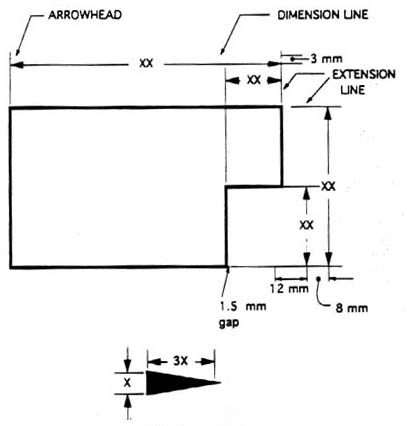
\includegraphics[width=2.4in]{fig/fig_dimensioned.jpg}
  \caption{Dimensioned Drawing}\label{fig_Dimensioned_Drawing}
\end{figure}

\begin{figure}
  \centering
  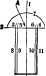
\includegraphics[width=0.3in]{fig/drawing-0111-2.jpg}
  \caption{bolt}\label{fig_bolt}
\end{figure}

\begin{figure}
  \centering
  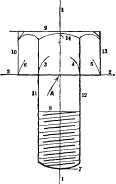
\includegraphics[width=0.4in]{fig/drawing-0112-1.jpg}
  \caption{bolt with a hexagon head}\label{fig_bolt1}
\end{figure}

\begin{figure}
  \centering
  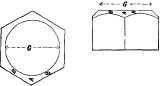
\includegraphics[width=1.1in]{fig/drawing-0121-1.jpg}
  \caption{nut}\label{fig_nut}
\end{figure}

\begin{figure}
  \centering
  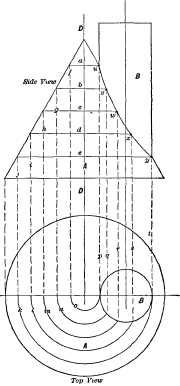
\includegraphics[width=0.9in]{fig/drawing-0189-1.jpg}
  \caption{a cylinder intersects a cone}\label{fig_projection}
\end{figure}

\subsection{Mechanics Base II}
This is a six-in-one course focus on mechanics design for non mechanics majors. The course talks about Planar Four-Bar Linkage, Cams, Statics, Mechanics of Materials, Shaft, Bearing, Gearing, as well as Tolerance and Fastener. I've learnt how to design a Axle or a gearbox, and how to choose bearings.

本课程主要讲述六个学科的主体内容,即理论力学、材料力学、机械原理、机械零件、仪器零件、公差,是非机类专业必修的一门主干课程。主要讲述机械中通用零、部件及常用机构的工作原理及设计方法。主要内容有静力学(Statics)、材料力学(mechanics of materials)、平面四连杆机构(Planar four-bar linkage)、齿轮传动(gearing)、凸轮(cams)、螺旋传动、轴(Axle)、轴承(bearing)、导轨(slide guide)、弹性元件(elastic element)、联接(Fastener)、公差(tolerance)。

\subsubsection{Planar four-bar linkage}
The synthesis, or design, of four bar mechanisms is important when aiming to produce a desired output motion for a specific input motion.

\paragraph{Grashof condition} If the sum of the shortest and longest link of a planar quadrilateral linkage is less than or equal to the sum of the remaining two links, then the shortest link (crank) can rotate fully with respect to a neighboring link.
\begin{figure}
  \centering
  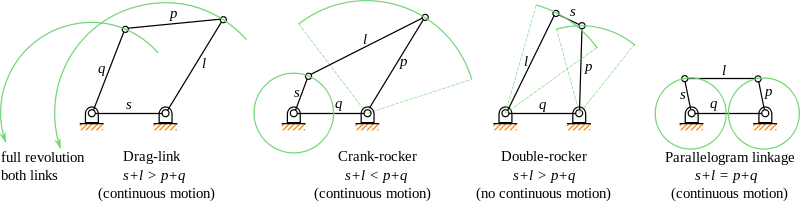
\includegraphics[width=4.5in]{fig/800px-Linkage_four_bar.svg.png}
  \caption{Types of four-bar linkages, s = shortest link, l = longest link. In the caption of the first figure, one must read s + l < p + q.}\label{fig_four_bar_linkage}
\end{figure}

\subsubsection{Cam}
A Cam is a machine component that either rotates or moves back and forth (reciprocates) to create a prescribed motion in a contacting element known as a follower. Cam systems can replace relatively complicated linkages in achieving desirable motion cycles.

\subsubsection{Mechanics of Materials}
Mechanics of Materials is a subject which deals with the behavior of solid objects subject to stresses and strains. Shear and bending moment diagrams are analytical tools used in conjunction with structural analysis to help perform structural design by determining the value of shear force and bending moment at a given point of a structural element such as a beam.

\begin{figure}
  \centering
  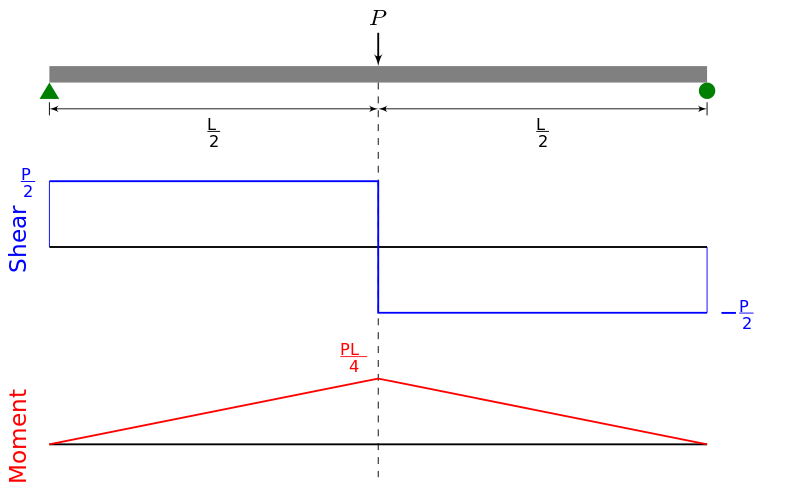
\includegraphics[width=4.2in]{fig/Shear_Moment_Diagram.svg.png}
  \caption{Shear and moment diagram for a simply supported beam with a concentrated load at mid-span.}\label{fig_Shear_Moment_Diagram}
\end{figure}

\subsubsection{Bearing}
The traditional method to estimate the life of the rolling-element bearings uses the basic life equation:
$$L_{10} = (C/P)^p \mbox{    }10^6 r$$

Where:

$L_{10}$ is the `basic life' (usually quoted in millions of revolutions) for a reliability of 90\%, i.e. no more than 10\% of bearings are expected to have failed

$C$ is the dynamic load rating of the bearing, quoted by the manufacturer

$P$ is the equivalent dynamic load applied to the bearing

$p$ is a constant: 3 for ball bearings, and 3.33 for roller bearings

\subsubsection{Gear}
A gear is a rotating machine part having cut teeth, which mesh with another toothed part in order to transmit torque.

Two or more gears working in tandem are called a transmission and can produce a mechanical advantage trough a gear ratio and thus may be considered a simple machine.

\paragraph{Gear Selection}
\begin{itemize}
  \item Pitch
  \item Face width
  \item Material
  \item Pressure angle
  \item \# of teeth
\end{itemize}

\paragraph{Worm gear} Worm-and-gear sets are a simple and compact way to achieve a high torque, low speed gear ratio.

\paragraph{Planetary Gear Trains}
\begin{figure}
  \centering
  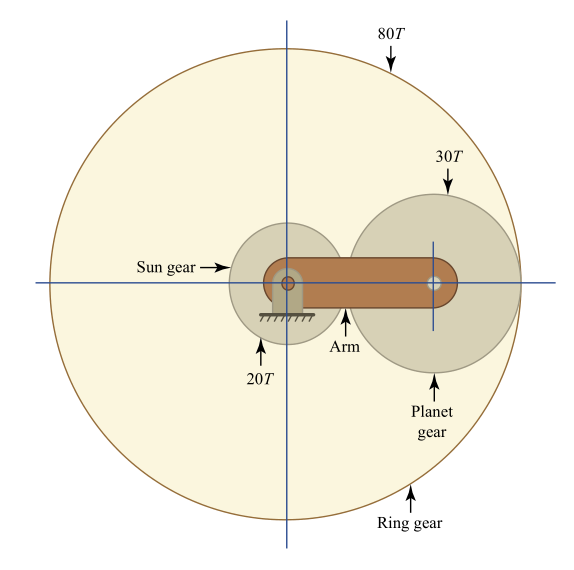
\includegraphics[width=3.2in]{fig/fig_planetary.png}
  \caption{Planetary Gear Trains}\label{fig_planetary}
\end{figure}

$$\mbox{Gear ratio   } e=\frac{n_L-n_A}{n_F-n_A}$$
where $n_L$: speed of last gear,

$n_A$: speed of arm,

$n_F$: speed of first gear(the sun)

\subsubsection{Coupling}
Couplings with parallel side keys are suitable for transfer of torsional moments, mostly in the same direction of rotation. Couplings with straight-sided splines are suitable for transfer of great, cyclical and shock torsional moments.

\begin{figure}
  \centering
  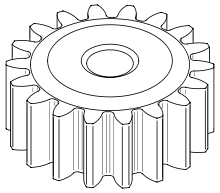
\includegraphics[width=1in]{fig/220px-Spur_Gear_12mm,_18t.svg.png}
  \caption{Spur Gear}\label{fig_spur}
\end{figure}
\begin{figure}
  \centering
  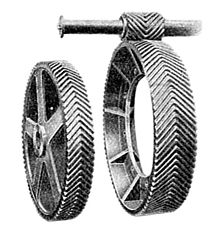
\includegraphics[width=1in]{fig/220px-Herringbone_gears_(Bentley,_Sketches_of_Engine_and_Machine_Details).jpg}
  \caption{Double helical}\label{fig_helical}
\end{figure}
\begin{figure}
  \centering
  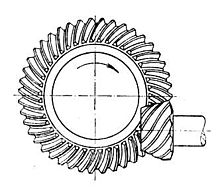
\includegraphics[width=1in]{fig/File-Sprocket35b.jpg}
  \caption{Bevel Gear}\label{fig_bevel}
\end{figure}
\begin{figure}
  \centering
  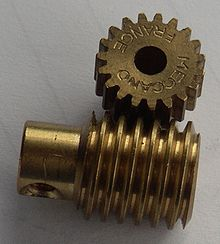
\includegraphics[width=1in]{fig/220px-Worm_Gear_and_Pinion.jpg}
  \caption{Worm gear}\label{fig_worm}
\end{figure}


\subsection{Sensing Technology and Its Applications}
In this course, I've got the basic knowledge of sensors, and several types of sensors, including resistance transducers, capacitor transducers, and inductance transducers, thermocouple, and optical sensors.

Sensors detect various physical parameters, and they are for gathering information, and for controlling systems.

A transducer is composed of Sensing element and Signal conditioning element.

\paragraph{Specifications}
\begin{itemize}
  \item Accuracy
  \item Linearity
  \item Sensitivity
  \item Repeatability
  \item Response time
\end{itemize}

\subsubsection{Resistance Transducers}
\paragraph{Strain Gauges} Resistance Strain Gauges are transducers which exhibit a change in electrical resistance in response to mechanical strain.

\paragraph{Resistance Temperature Detector (RTD)}
The RTD element is made from a pure material, typically platinum, nickel or copper. RTDs in industrial applications are rarely used above $660^{\circ}C$.

For Platinum RTD: $R_t=R_0[1+At+Bt^2]$
\subparagraph{Advantage}
\begin{itemize}
  \item High accuracy
  \item Low drift
  \item Wide operating range
  \item Suitability for precision applications
\end{itemize}

\subsubsection{Thermocouples}
All electrically conducting materials produce a thermal e. m. f., this is called the \emph{Seebeck effect}. When two different materials are connected to create a $T^\circ C$, a voltage is generated.

Advantages:
\begin{itemize}
  \item Capable of being used to directly measure temperatures up to $2600^{\circ}C$.
\end{itemize}

Disadvantages:
\begin{itemize}
  \item requires two temperatures be measured
  \item not linear
\end{itemize}

\subsubsection{Capacitor Transducers}
The capacitive transducer is used extensively for the measurement of displacement, pressure etc. The capacitive transducer or sensor is nothing but the capacitor with variable capacitance.
$$C=\frac{\varepsilon S}{d}=C_0+\Delta C = \frac{\varepsilon S}{d-\Delta d}=\frac{C_0}{1-\frac{\Delta d}{d}}$$

\begin{figure}
  \centering
  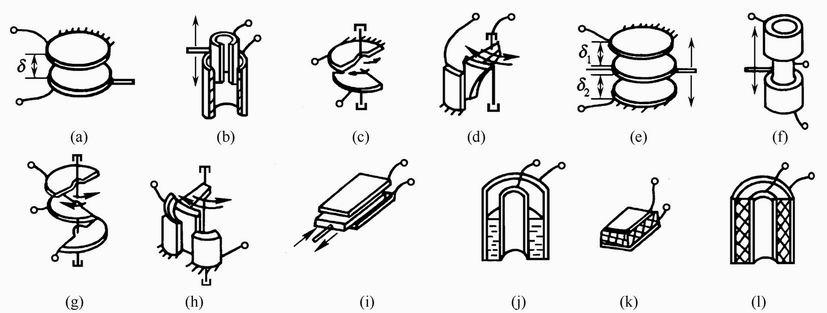
\includegraphics[width=4.2in]{fig/fig_capacitor.jpg}
  \caption{Capacitor Transducers}\label{fig_capacitor}
\end{figure}

Depending on the parameter that changes for the capacitive transducers, they are of three types as mentioned below.
\begin{itemize}
  \item Changing Dielectric Constant type of Capacitive Transducers
  \item Changing Area of the Plates of Capacitive Transducers
  \item Changing Distance between the Plates of Capacitive Transducers
\end{itemize}

Advantages:
\begin{itemize}
  \item It produces an accurate frequency response to both static and dynamic measurements.
\end{itemize}

Disadvantages:
\begin{itemize}
  \item An increase or decrease in temperature to a high level will change the accuracy of the device.
  \item As the lead is lengthy it can cause errors or distortion in signals.
\end{itemize}

\subsubsection{Inductive Transducer}
This type of transducer is used for finding the linear displacement in terms of voltage or other digital parameters.

Inductive transducers can be classified as follows:
\begin{enumerate}
  \item Variable self inductance: single coil, two coil
  \item Variable mutual inductance: simple two, three coil
  \item Variable reluctance: moving iron, moving coil, moving magnet
\end{enumerate}

\begin{figure}
  \centering
  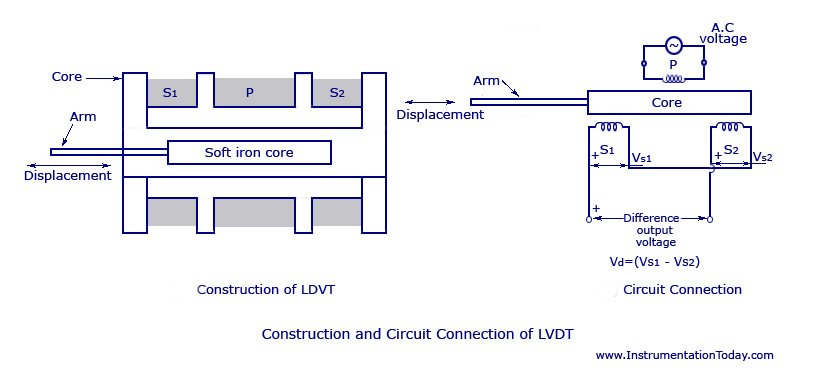
\includegraphics[width=4.2in]{fig/LVDT-Construction.jpg}
  \caption{Linear Voltage Differential Transformer (LVDT) Construction}\label{fig_LVDT}
\end{figure}

LVDT Advantages:
\begin{itemize}
  \item Maintains a linear relationship between the voltage difference output and displacement from each position of the core for a displacement of about 4 millimeter.
  \item Produces low hysteresis and thus has easy repeatability.
\end{itemize}

LVDT Disadvantages:
\begin{itemize}
  \item The whole circuit is to be shielded as the accuracy can be affetced by external magnetic field.
  \item A demodulator will be needed to obtain a d.c output.
  \item The efficiency of the device is easily affected by temperature.
\end{itemize}

\begin{figure}
  \centering
  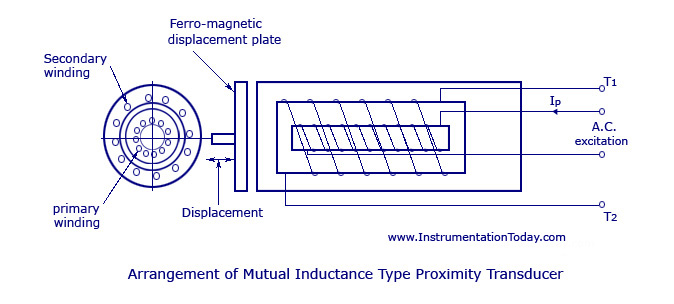
\includegraphics[width=4.2in]{fig/Proximity-Inductive-Transduccers.jpg}
  \caption{Proximity Inductive Transducers}\label{fig_proximity_inductive}
\end{figure}


\begin{figure}
  \centering
  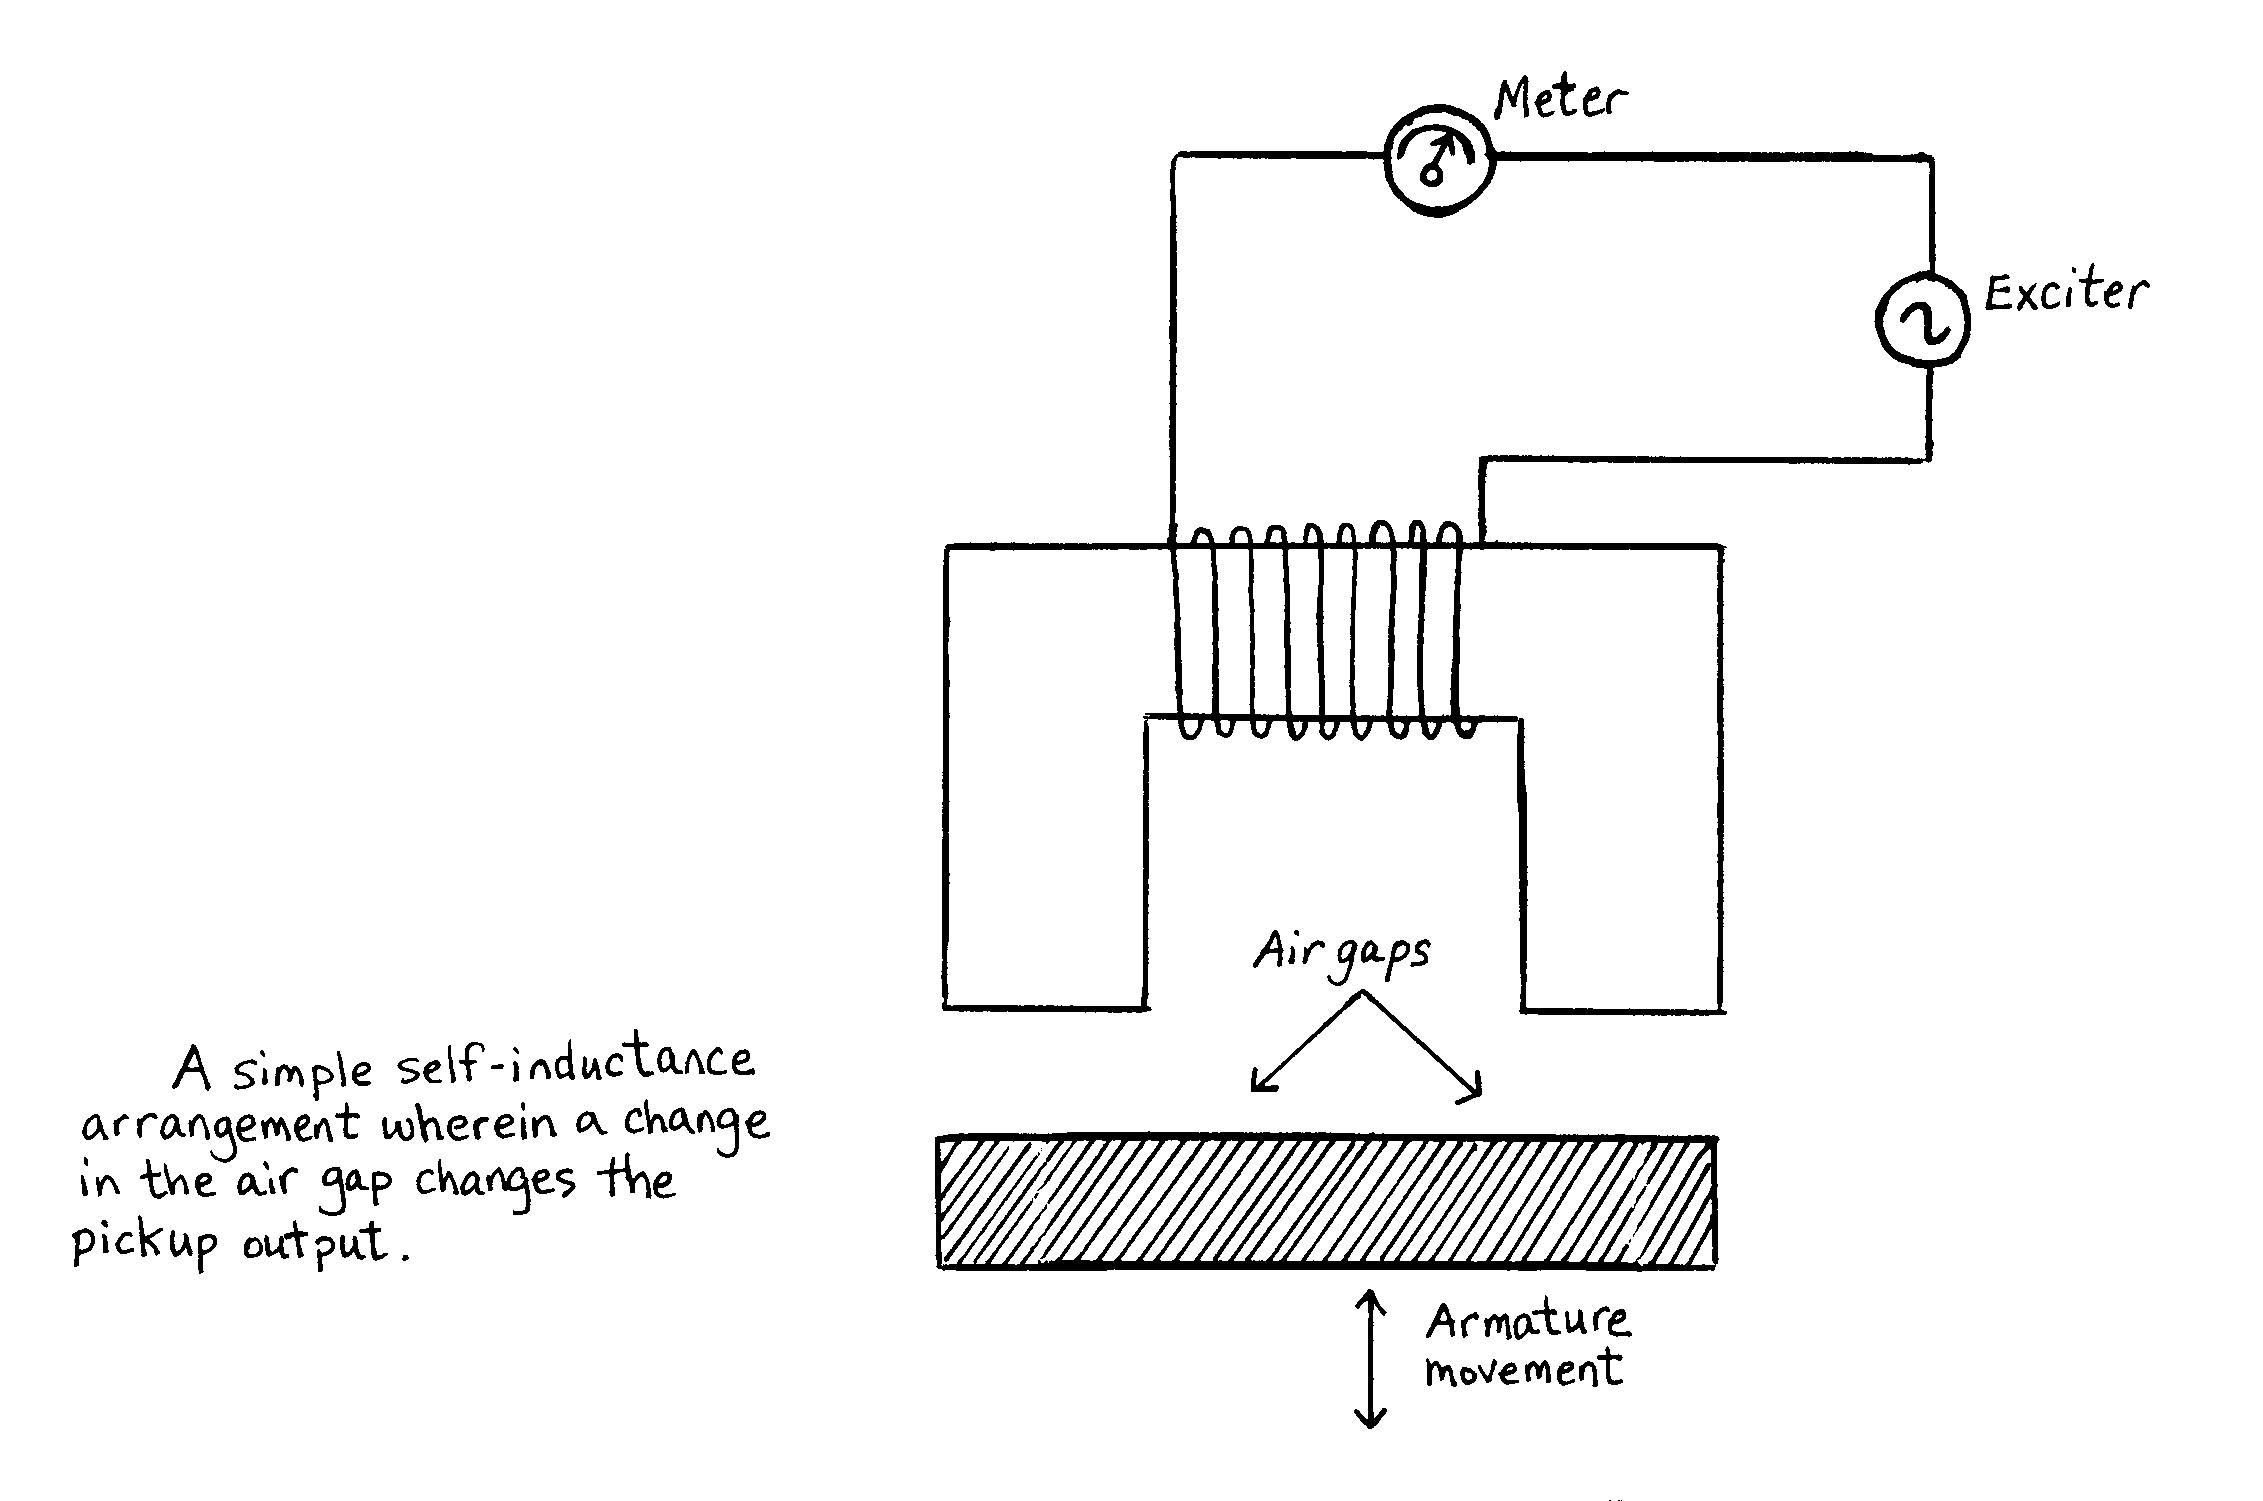
\includegraphics[width=3.5in]{fig/Image22.png}
  \caption{Simple self inductance arrangement}\label{fig_inductance}
\end{figure}

\paragraph{Magnetic Transducers}
The Hall effect is the production of a voltage difference (the Hall voltage) across an electrical conductor, transverse to an electric current in the conductor and a magnetic field perpendicular to the current.

$F_L=evB$, $F_E=-eE_H=-eU_H/b$,

when $F_L+F_E=0$, $vB=U_H/b$

as $j=-nev$, $I=jbd=-nevbd$, and $v=-I/(nebd)$.

Thus:
$$U_H=-\frac{BI}{ned}=R_H\frac{IB}{d}=k_HIB$$
where $R_H$ is Hall coefficient.

Advantages:
\begin{itemize}
  \item not affected by ambient conditions, such as dust, humidity, and vibrations
  \item do not have contact with neighboring mechanical parts
  \item A high speed operation is possible.
\end{itemize}

Disadvantages:
\begin{itemize}
  \item Temperature affects the electrical resistance of the element and the mobility of majority carriers and also the sensitivity of Hall Effect sensors.
  \item An offset voltage occurs when there are physical inaccuracies and material non-uniformities.
\end{itemize}

\begin{figure}
  \centering
  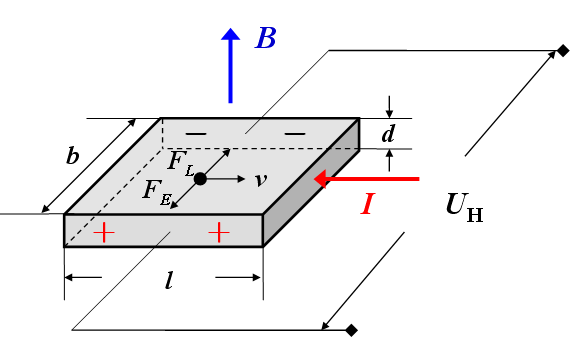
\includegraphics[width=2.5in]{fig/fig_Hall.png}
  \caption{Hall Effect}\label{fig_hall}
\end{figure}

\subsubsection{Optic Transducers}
\begin{itemize}
  \item Photoemissive (Photodiodes/Phototransistors)
  \item Photoconductive (Photoresistors)
  \item CCD (Charge-coupled device)
\end{itemize}

\subsection{Project Design in Fundamentals of Mechanics}
\subsection{Engineering Training (Metalworking Practice)}
\subsection{Engineering Training (Electronic Processing Practice)}
In the practice, I've build up a radio by myself. The first thing to learn is Schweissen, then printed circuit board. After that, I placed the discrete components on the board, and began to schweissen. Finally, I managed to hear sound from the radio. 